\documentclass[a4paper]{article}
\usepackage{vmargin}
\usepackage[utf8]{inputenc}
\usepackage[english]{babel}

\usepackage{array}
\usepackage{enumerate}
\usepackage{multicol}
\usepackage{multirow}

\usepackage{Sweave}
\usepackage{vmargin}

\setmarginsrb{1.5cm}{1cm}{1.5cm}{1cm}{1cm}{1cm}{1cm}{1cm}

\usepackage{hyperref}
\hypersetup{colorlinks,%
            citecolor=black,%
            filecolor=black,%
            linkcolor=black,%
            urlcolor=blue}

\DefineVerbatimEnvironment{Sinput}{Verbatim}{formatcom={\color[rgb]{0.56,0,0}}}
\DefineVerbatimEnvironment{Soutput}{Verbatim}{formatcom={\color[rgb]{0,0,0.56}}} 



\begin{document}
\thispagestyle{empty}
\setkeys{Gin}{width=100pt}
\begin{minipage}{0.6\linewidth}
\begin{center}
\begin{large}
The University of Auckland\\
\end{large}
\end{center}
\end{minipage}


\setkeys{Gin}{width=30pt}
\begin{center} 
\vspace{270 pt}
\begin{Huge}
\hrule
\vspace{2pt}
\hrule
\vspace{5pt}
Tutorial R package \texttt{phyloland}\\
\vspace{5pt}
\hrule
\vspace{2pt}
\hrule
\end{Huge}
\end{center}
\begin{flushright}
\begin{Large}
\textbf{Marie Paturel, Louis Ranjard}\\
\end{Large}
\end{flushright}
\vspace{250pt}
\begin{center}
\today
\end{center}
\vspace{35pt}
\newpage

\section*{Introduction}
\setkeys{Gin}{width=15pt}
\hspace{12pt} This tutorial illustrates the use of the \texttt{phyloland} R package.
The phylogeny of Hawaiian katydids {\it Banza} genus species is used to analyse the history of dispersal events that led to the colonisation of the archipelago.
In particular, the effect of competitive exclusion and limited dispersal on dispersals will be investigated using in a statistical phylogeographic framework (see the package documentation for more information).
Examples of the use of the main functions of the package are presented.\\

\tableofcontents



\newpage
\setlength\abovecaptionskip{-12pt}
\section{Data set: Hawaiian katydids}
\begin{itemize}
\renewcommand{\labelitemi}{$\bullet$}
\item The geological history of the Hawaiian archipelago is well known - new islands are created over an undersea magma source (hotspot) laying beneath the northwestward-moving Pacific tectonic plate.
\item The Banza genus (Hawaiian katydids) shows evidence for island radiation with different species inhabiting each island which is predicted to follow a simple progression rule: species from older islands are basal to those from younger islands therefore the sequence of colonisation follows the ages of the islands.
\item The model was fitted to the posterior distribution of trees obtained from BEAST v1.7.0 using the COI sequences from 21 individuals\cite{hawaii}.
Alternatively, the consensus tree was used to fit the model (see below).
\end{itemize}
\setkeys{Gin}{width=400pt}
\begin{figure}[h!]
\begin{center}
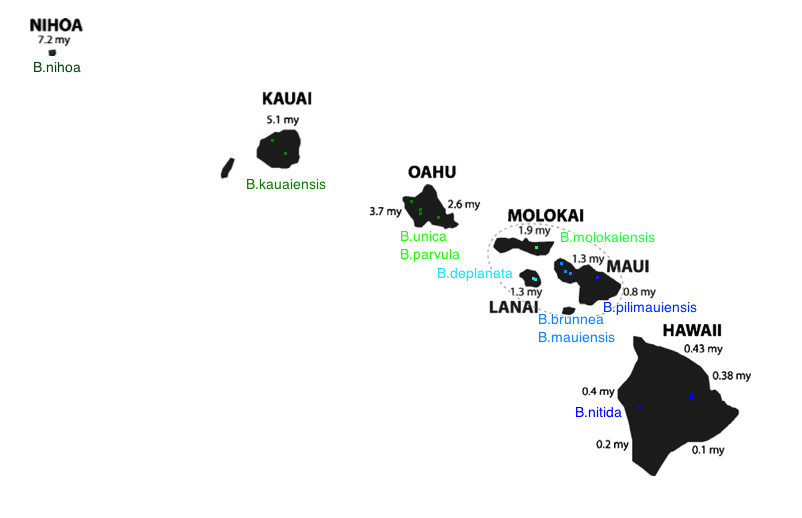
\includegraphics{figures/hawaii.png}
\caption{Hawaii archipelago with the tip locations.
Adapted from Shapiro et al. (2006)\cite{hawaii}}
\end{center}
\end{figure}


\newpage
\section{MCMC}
\hspace{12pt} The consensus phylogenetic tree is read in the file "tree\_Banza.nex" or "tree\_Banza\_posterior.nex" (\texttt{fileTREES}) and the 2-dimensional location coordinates (latitudes and longitudes in decimal) is in the file "locations\_Banza.txt" (\texttt{fileDATA}).
The file "tree\_Banza\_posterior.nex" is the posterior distribution of phylogenies generated by Beast and the "tree\_Banza.nex" contains the consensus tree computed from that distribution.
The Markov Chain is set to run for 100,000 steps (\texttt{num\_step=1e5}) with the model parameters and internal tree nodes locations sampled every 100 steps (\texttt{freq=1e2}).
The expected sample size limit is set to a large value (\texttt{ess\_lim\_step=1e6}) so that the chain will run until the requested number of steps.
The output files will be named using the pattern "Banza" (\texttt{id\_filena}).
The parameter \texttt{names\_locations} contains the names of the five main Hawaiian Islands: Nihoa, Kauai, Oahu, Maui Nui (grouping Molokai, Lanai and Maui) and Hawaii.
\texttt{names\_locations} must contain the same number of elements as the number of tips in the tree.
If omitted, the tree file tip names of the first occurences of each geographic location, as determined by their coordinates in \texttt{fileDATA}, will be used.


\begin{Schunk}
\begin{Sinput}
> library(phyloland)
> names_locations = c("Maui_Nui", "Maui_Nui", "Maui_Nui", "Maui_Nui", "Kauai", "Kauai",
 "Maui_Nui", "Maui_Nui", "Maui_Nui", "Maui_Nui", "Nihoa", "Nihoa", "Hawaii", "Hawaii",
  "Hawaii", "Oahu", "Oahu", "Maui_Nui", "Maui_Nui", "Oahu", "Oahu")
> Banza = PLD_interface(fileTREES="tree_Banza_posterior.nex", fileDATA="locations_Banza.txt",
 num_step=1e5, freq=1e2, ess_lim=1e6, names_locations=names_locations)
\end{Sinput}
\end{Schunk}

Alternatively, use a consensus phylogeny

\begin{Schunk}
\begin{Sinput}
> Banza = PLD_interface(fileTREES="tree_Banza.nex", fileDATA="locations_Banza.txt",
 num_step=1e5, freq=1e2, ess_lim=1e6, names_locations=names_locations)
\end{Sinput}

\begin{Soutput}
[1] "sigma upper limit 1 : 13.7878461374569"
[1] "sigma upper limit 2 : 49.7703754827825"
[1] "100     6.8939     24.8852     720.2046     262.0676     -Inf    "
...
[1] "98900     8.0001     4.2011     2.2776     23.7270     15.0430    "
[1] "99000     0.7495     7.2136     0.7077     95.8285     19.7028    "
[1] "             Sigma        Sigma        Lambda      Tau"
[1] "ess:     340.1152     330.0475     314.2442    316.3114"
[1] "99100     9.3240     3.6189     0.4886     95.4336     16.1921    "
[1] "99200     6.7828     1.5855     2.6893     21.0914     10.0696    "
[1] "99300     4.8725     1.9596     1.3347     28.8024     3.9171    "
[1] "99400     4.6244     3.7325     0.8217     49.6006     14.0936    "
[1] "99500     2.0673     4.8015     1.3518     55.0591     19.7023    "
[1] "99600     0.5474     9.5637     0.7763     78.1568     14.4342    "
[1] "99700     1.0796     12.9417     0.6076     103.7920     17.8745    "
[1] "99800     0.7235     22.4217     1.2566     37.7616     10.3022    "
[1] "99900     0.6654     34.8823     0.7434     83.7312     19.2065    "
[1] "100000     8.7321     4.2144     2.7987     18.9420     15.0183    "
[1] "             Sigma        Sigma        Lambda      Tau"
[1] "ess:     343.1347     332.6158     317.5541    319.5934"
\end{Soutput}
\end{Schunk}

First, the limits on sigma in the space are computed.
Second, the sampled values for each parameters are printed as well as the log likelyhood in the following order:\\
sample number, sigma dimension 1, sigma dimension 2, lambda, tau, log-likelihood.
The estimated sample sizes (\texttt{ess}) are calculated every 10 samples.

The estimation will stop when \texttt{num\_step} is reached or when the ess of all estimated parameters equal \texttt{ess\_lim}.
An object \texttt{phyloland} is returned, containing the sampled locations, the tip names and the space with the locations.

\newpage
\section{Model parameters}
\hspace{12pt} The values of the parameters of the MCMC are recorded in the file "tracer\_Banza.log", while the internal locations are recorded in "loc\_Banza.log".
The posterior distribution of the parameters are summarized in the file "phyloland\_Banza.nex".
%These files can be read to plot the posterior distribution of each parameter.
The posterior distribution of each parameter can be plotted using the following commands

\begin{Schunk}
\begin{Sinput}
> mcmc_log = Banza$mcmc[[1]]
> x11(); par(mfrow=c(2,2))
> hist(mcmc_log[,2],40,xlab="sigma 1",main="sigma 1"); abline(v=Banza$mcmc[[8]][1],lwd=2,col="red")
> hist(mcmc_log[,3],40,xlab="sigma 2",main="sigma 2"); abline(v=Banza$mcmc[[8]][2],lwd=2,col="red")
> hist(log(mcmc_log[,4]),40,xlab="lambda",main="lambda"); abline(v=log(1),lwd=2,col="red")
> hist(mcmc_log[,5],40,xlab="tau",main="tau")
\end{Sinput}

\begin{Soutput}

\end{Soutput}
\end{Schunk}
%alternatively to load another run
%> mcmc_log = read.csv("tracer_Banza.log",sep="\t")
\hspace{12pt}A single figure is created showing the posterior distribution with the calculated limits on sigma, below which limited dispersal is inferred, and the neutral value of lambda, i.e. 1.
Smaller values of lambda suggest that secondary colonisation are somehow prevented while larger value indicate that occupied location of space are colonised more easily than empty locations.\\

\setkeys{Gin}{width=400pt}
\begin{figure}[h!]
\begin{center}
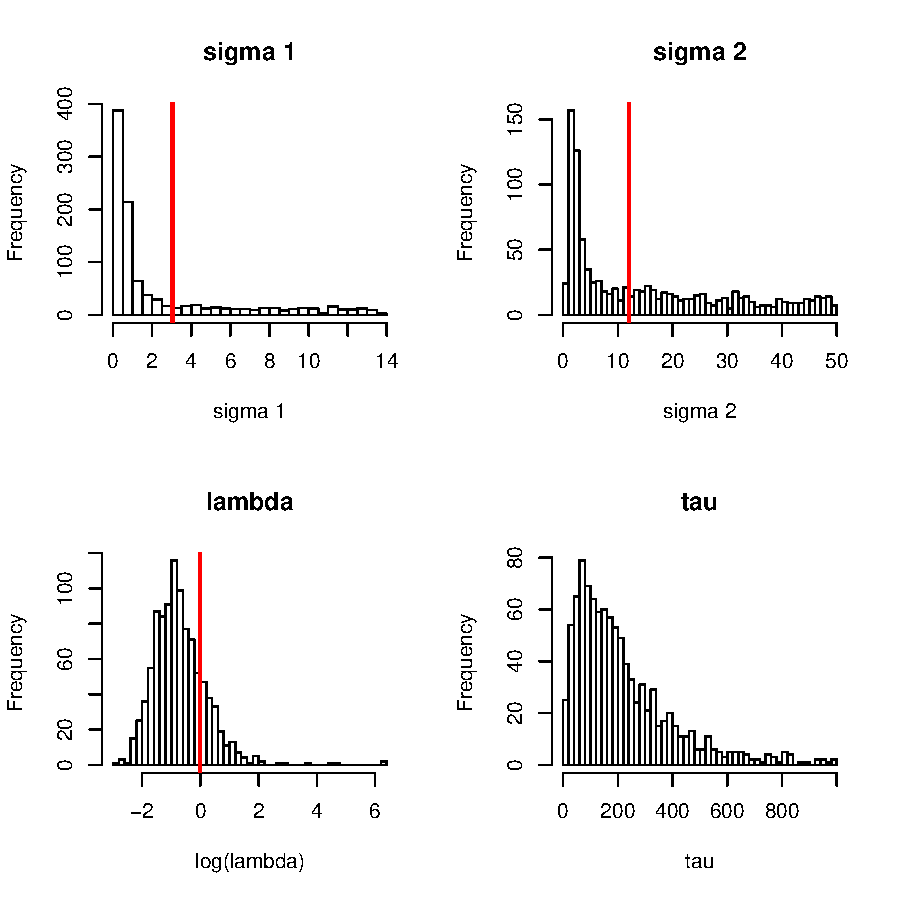
\includegraphics[width=.7\textwidth]{figures/post_dist.pdf}
\caption{Model parameter posterior distributions.}
\end{center}
\end{figure}

It appeared that the dispersal along sigma 1 dimension, i.e. latitude - first column of the file "locations\_Banza.txt" , are more restricted than along the longitude axis.
This results is expected as the Hawaiian islands are localised on similar latitudes (19N-22N).
The range of longitude coordinates between islands is greater, therefore dispersals corresponded to larger distances on the longitudinal axis leading to a greater estimate for sigma along that axis.
The estiamtes of lambda indicate that secondary colonisation were prevented, suggesting that competitive exclusion may have occured in the colonisation history of the archipelago.

\newpage
\section{Display tree}
\hspace{12pt} A tree with the locations of internal nodes sampled at a particular step (\texttt{sub\_sample}) of the MCMC can be plotted using the phyloland object Banza (\texttt{x = Banza}).
\begin{Schunk}
\begin{Sinput}
> PLD_plot_trees(x = Banza, sub_sample = 5)
\end{Sinput}

\begin{Soutput}
[1] "tree 5"
[1] "((((((deplanataA:0.01984498998,deplanataB:0.01984498998)Maui_Nui:2.613
393913,(molokaiensisA:0.02228635824,molokaiensisB:0.02228635824)Maui_Nui:2.
610952545)Maui_Nui:0.6309764856,((parvulaA:0.932186106,parvulaB:0.932186106
)Oahu:0.7511685962,(kauaiensisA:0.3811763191,kauaiensisB:0.3811763191)Kauai
:1.302178383)Oahu:1.580860687)Oahu:1.086280558,((nitidaC:1.974160409,(nitid
aA:0.6608291397,nitidaB:0.6608291397)Hawaii:1.313331269)Hawaii:0.4692204906
,((brunneaA:0.2413846814,brunneaB:0.2413846814)Maui_Nui:1.957752707,((pilim
auiensisA:0.193703458,pilimauiensisB:0.193703458)Maui_Nui:0.2634806302,(mau
iensisA:0.06130037131,mauiensisB:0.06130037131)Maui_Nui:0.395883717)Maui_Nu
i:1.741953301)Maui_Nui:0.244243511)Hawaii:1.907115047)Oahu:0.8879125883,(un
icaA:1.546870539,unicaB:1.546870539)Oahu:3.691537996)Oahu:2.736223477,(niho
aA:0.02267346127,nihoaB:0.02267346127)Nihoa:7.951958551)Oahu;"
\end{Soutput}
\end{Schunk}
\hspace{12pt}The Newick format is printed and the tree with the internal locations and the tip names.\\

\setkeys{Gin}{width=350pt}
\begin{figure}[h!]
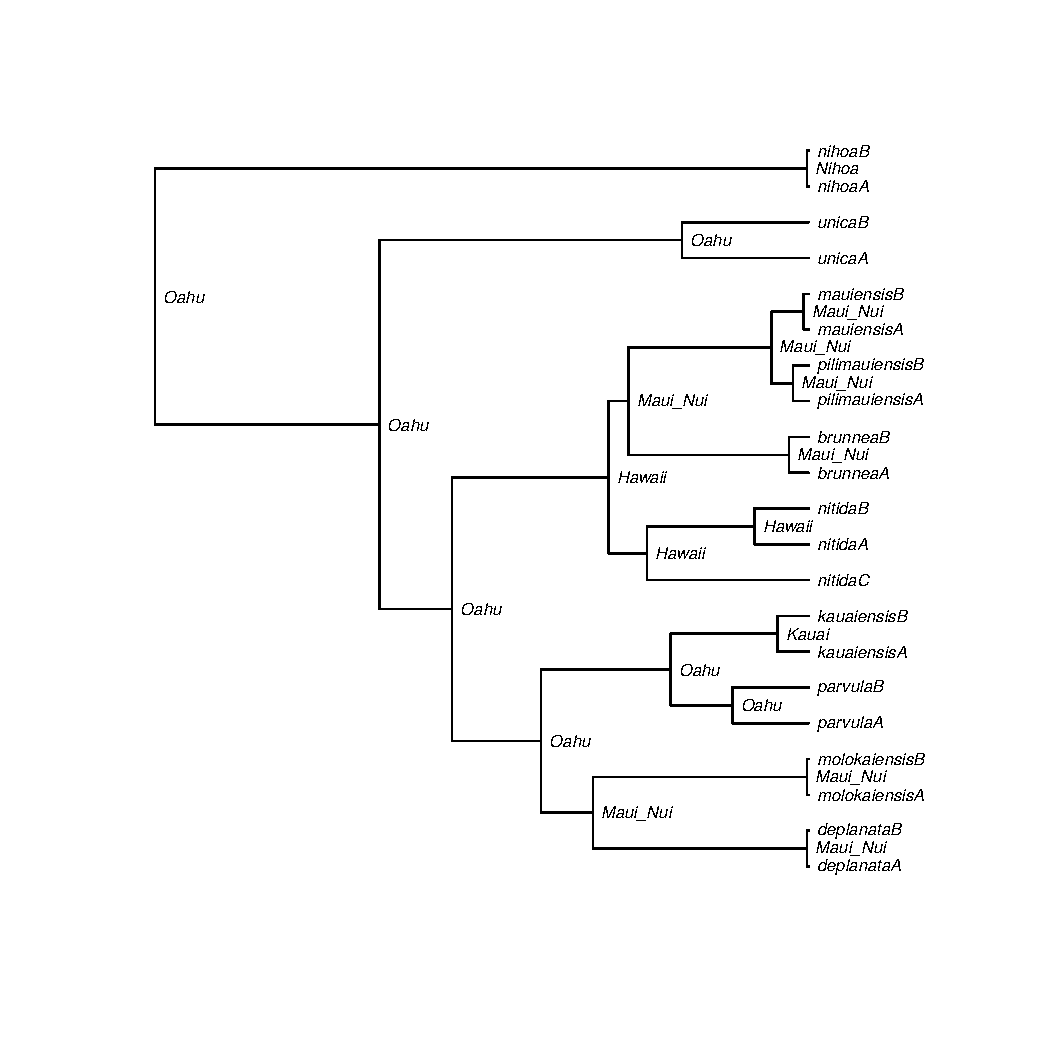
\includegraphics[]{figures/tree_5.pdf}
\caption{Tree at step 5}
\end{figure}

At different step of the MCMC, different locations for the internal nodes are sampled.
For example, the location of the root of the tree is different at steps 6 and 8:
\begin{Schunk}
\begin{Sinput}
> PLD_plot_trees(x = Banza, sub_sample = c(20, 1000), one_plot = TRUE)
\end{Sinput}
\begin{Soutput}
[1] "tree 20"
[1] "((nihoaA:0.02682250713,nihoaB:0.02682250713)Nihoa:15.37518602,((unicaA
:1.516171475,unicaB:1.516171475)Oahu:4.505519854,((((molokaiensisB:0.023296
19177,molokaiensisA:0.02329619177)Maui_Nui:3.319490667,(deplanataB:0.021918
18003,deplanataA:0.02191818003)Maui_Nui:3.320868679)Maui_Nui:0.5968550136,(
(parvulaA:1.080851141,parvulaB:1.080851141)Oahu:0.8046901679,(kauaiensisA:0
.4046608492,kauaiensisB:0.4046608492)Kauai:1.480880459)Kauai:2.054100564)Ma
ui_Nui:1.437976587,((nitidaC:2.389908883,(nitidaB:0.7288534034,nitidaA:0.72
88534034)Hawaii:1.66105548)Hawaii:0.5041477603,(((pilimauiensisA:0.20974455
51,pilimauiensisB:0.2097445551)Maui_Nui:0.2654363599,(mauiensisB:0.06288956
014,mauiensisA:0.06288956014)Maui_Nui:0.4122913548)Maui_Nui:1.937111341,(br
unneaB:0.2517520192,brunneaA:0.2517520192)Maui_Nui:2.160540237)Maui_Nui:0.4
817643872)Maui_Nui:2.483561816)Maui_Nui:0.6440728698)Oahu:9.380317199)Oahu;
"
[1] "tree 1000"
[1] "((nihoaA:0.02682250713,nihoaB:0.02682250713)Nihoa:15.37518602,((unicaA
:1.516171475,unicaB:1.516171475)Oahu:4.505519854,((((molokaiensisB:0.023296
19177,molokaiensisA:0.02329619177)Maui_Nui:3.319490667,(deplanataB:0.021918
18003,deplanataA:0.02191818003)Maui_Nui:3.320868679)Maui_Nui:0.5968550136,(
(parvulaA:1.080851141,parvulaB:1.080851141)Oahu:0.8046901679,(kauaiensisA:0
.4046608492,kauaiensisB:0.4046608492)Kauai:1.480880459)Oahu:2.054100564)Oah
u:1.437976587,((nitidaC:2.389908883,(nitidaB:0.7288534034,nitidaA:0.7288534
034)Hawaii:1.66105548)Hawaii:0.5041477603,(((pilimauiensisA:0.2097445551,pi
limauiensisB:0.2097445551)Maui_Nui:0.2654363599,(mauiensisB:0.06288956014,m
auiensisA:0.06288956014)Maui_Nui:0.4122913548)Maui_Nui:1.937111341,(brunnea
B:0.2517520192,brunneaA:0.2517520192)Maui_Nui:2.160540237)Maui_Nui:0.481764
3872)Maui_Nui:2.483561816)Oahu:0.6440728698)Oahu:9.380317199)Oahu;"
\end{Soutput}
\end{Schunk}

\indent Both trees (Newick format) are printed and displayed with their internal and tip locations on the same figure.\\
\setkeys{Gin}{width=400pt}
\begin{figure}[h!]
\begin{center}
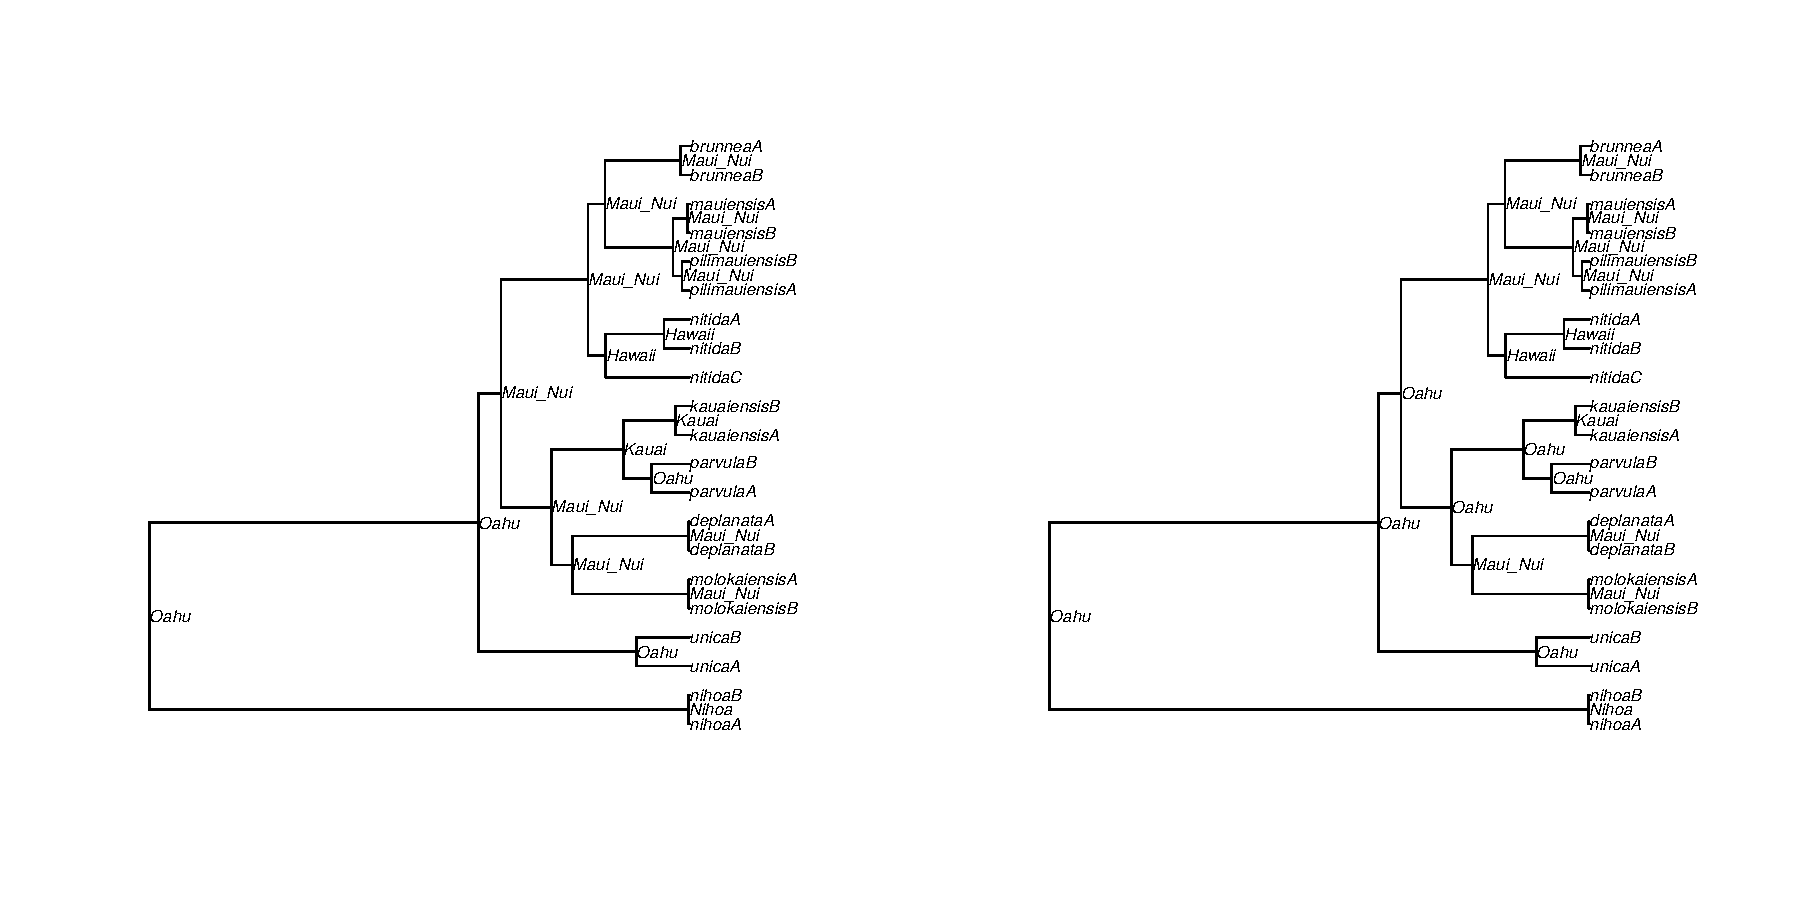
\includegraphics[width=.9\textwidth]{figures/tree_20_1000_Banza.pdf}
\caption{Trees at steps 20 \& 1000}
\end{center}
\end{figure}

\indent When using a posterior distribution of trees, the sampled tree have varying topologies.\\
\setkeys{Gin}{width=400pt}
\begin{figure}[h!]
\begin{center}
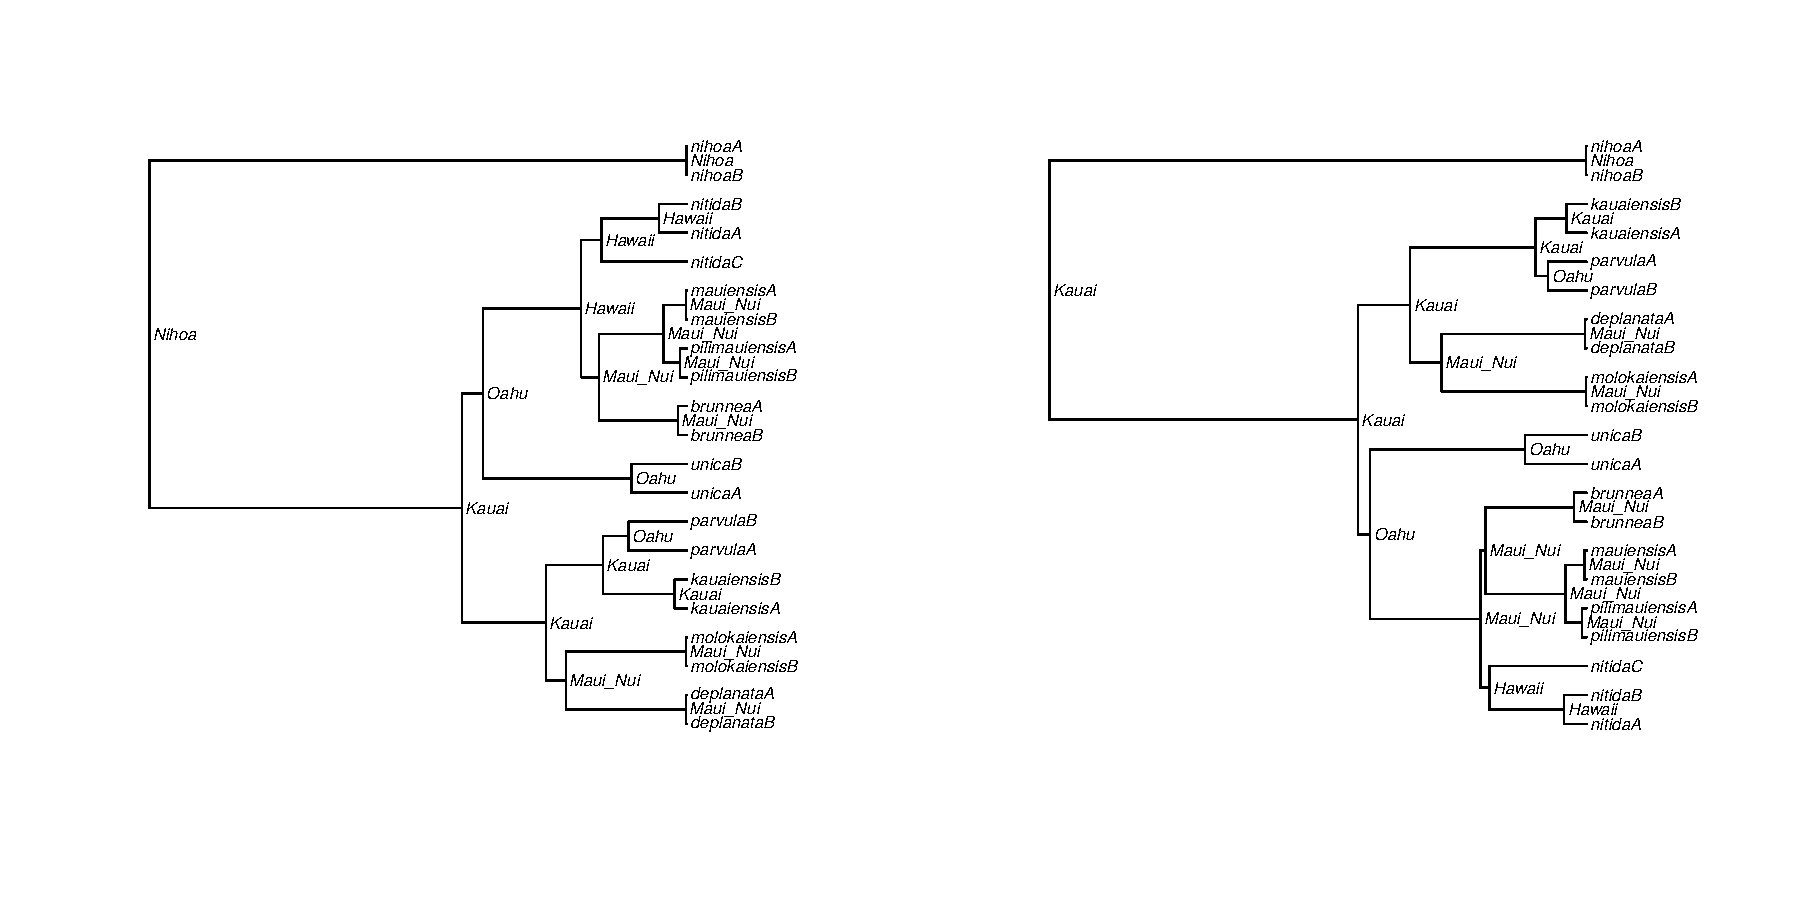
\includegraphics[width=.9\textwidth]{figures/tree_20_1000_Banzap.pdf}
\caption{Trees at steps 20 \& 1000}
\end{center}
\end{figure}

\setlength\abovecaptionskip{0pt}
\newpage
\section{Location of the Most Recent Common Ancestor of a set of tips}
\hspace{12pt} The function \texttt{PLD\_loc\_mrca} can be used to infer the geographic location of the Most Recent Common Ancestor of all the tips of the tree.
The parameters of the function are the phyloland object Banza (\texttt{x = Banza}), all the tips are selected (tips = Banza\$tips) and all the trees are taken into account (\texttt{sub\_sample = 0}) and the distribution of the locations is plotted as a barplot (\texttt{plot\_distrib = TRUE}).
The coordinates as well as sampled frequencies of each location for the root of the tree are stored in the object \texttt{locations}.

\begin{Schunk}
\begin{Sinput}
> locations <- PLD_loc_mrca(x = Banza, tips = Banza$tips, sub_sample = 0, plot_distrib = TRUE)
> locations$frequencies
\end{Sinput}
\end{Schunk}

\begin{Soutput}
         Dimension1 Dimension2 Frequency
Kauai      22.06444   159.5456     0.458
Nihoa      23.06222   161.9261     0.374
Oahu       21.43688   158.0524     0.122
Maui_Nui   20.90532   156.6499     0.043
Hawaii     19.73620   155.6069     0.003

\end{Soutput}

%Note the the Hawaii Island was not sampled as the location of ancestral population.
The posterior distribution of the locations of the MRCA indicates a stronger support for Kauai and Nihoa Islands as source population.
%However, this needs to be corrected by the fact that each island was not sampled evenly, e.g. Oahu Island-4 individuals and Nihoa-2 individuals, which could have affected these results.
While uncertainty remains about the origin of the diversification of the genus Banza in the Hawaiian archipelago, it is likely that one of these islands hosted the source population of most of the individuals sampled in this study.

\newpage
\section{Dispersal times}
\hspace{12pt}The distribution of the times of the first dispersals to each different island of the archipelago can be plotted.
The functions \texttt{PLD\_stat\_mig} and \texttt{PLD\_plot\_stat\_mig} use the phyloland object Banza (\texttt{x = Banza}) and allow to plot the corersponding distributions.
To reduce the computation time, only the first 1,000 trees with locations (\texttt{sub\_sample = 1:1000}) were taken into account.
The first dispersal only to each location are considered (\texttt{first = TRUE}).
\begin{Schunk}
\begin{Sinput}
> stat = PLD_stat_mig(x = Banza, sub_sample = 1:1000, first = TRUE)
> PLD_plot_stat_mig(timemat = stat$timemat, color = NA, xy_legend = NA)
\end{Sinput}
\end{Schunk}

\setkeys{Gin}{width=400pt}
\begin{figure}[h!]
\begin{center}
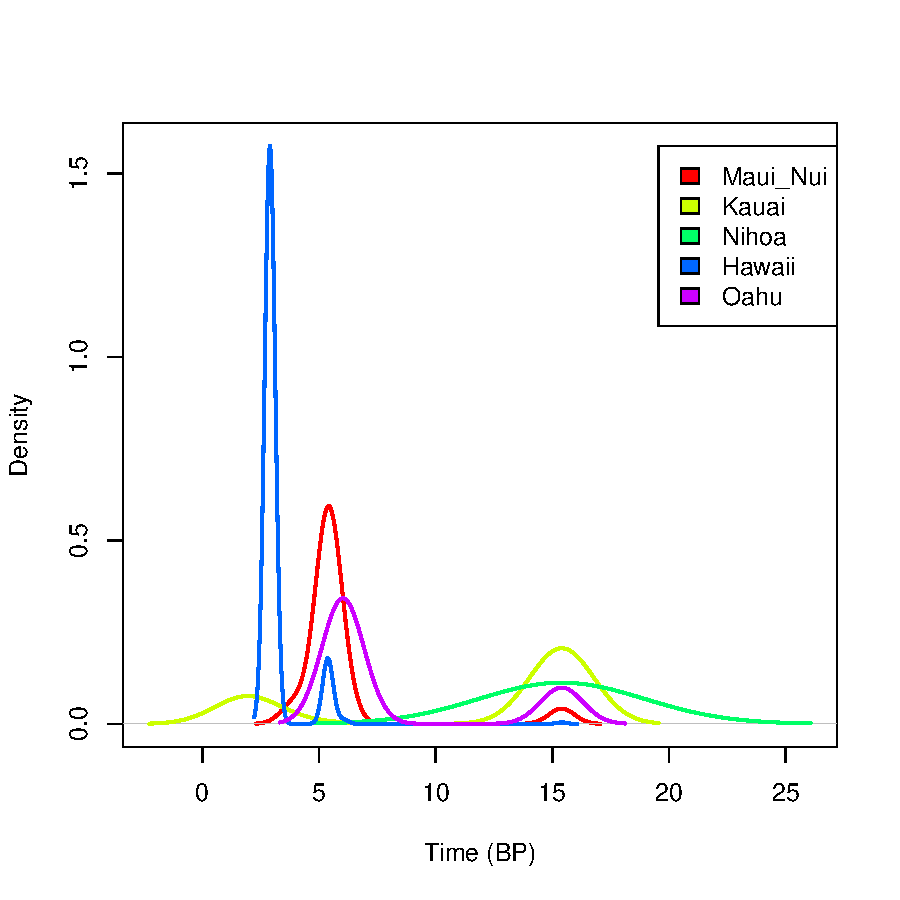
\includegraphics[width=.9\textwidth]{figures/timemig.pdf}
\caption{Density plots of the dispersal times for each location}
\end{center}
\end{figure}

Consistency between the estimated time of dispersals to the different Hawaiian islands and the geological estimates of their formation can be observed.
The oldest islands seem to have been colonized first and the youngest islands seem to have been colonized the most recently.
However, one can observe that dispersal times are all older than the geological formations of the corresponding islands.
This result can potentially be caused by an underestimate of the mutation rate in that genus\cite{hawaii}.

\newpage
\begin{thebibliography}{9}
   \bibitem{hawaii}
        L.H. Shapiro, J.S. Strazanac,  G.K. Roderick.
          \emph{Molecular phylogeny of Banza (Orthoptera: Tettigoniidae), the endemic katydids of the Hawaiian Archipelago}.
          Mol Phylogenet Evol. 2006 Oct;41(1):53-63. Epub 2006 Apr 25.
\end{thebibliography}

\end{document}
